\nonstopmode
\documentclass[master=cws,masteroption=gs]{kulemt}
\setup{title={Configuratieafhankelijkheden gebruiken om gedistribueerde applicaties effici\"ent te beheren in een hybride cloud},
  author={Harm De Weirdt},
  promotor={Prof.\,dr.\,ir.\ Wouter Joosen},
  assessor={Ir.\,W. Eetveel\and W. Eetrest},
  assistant={Ir.\ Bart Vanbrabant}}
% De volgende \setup mag verwijderd worden als geen fiche gewenst is.
\setup{filingcard,
    translatedtitle={Configuratieafhankelijkheden gebruiken om gedistribueerde applicaties effici\"ent te beheren in een hybride cloud},
  udc=T134, %TODO: checken
  shortabstract={
      \begin{description}
          \item[Context] \hfill \\ Om IT infrastructuren efficient te beheren wordt er gebruik gemaakt van configuratiebeheergereedschappen. Deze gereedschappen zijn model gebaseerd, waarbij het model de gewenste toestand van de configuratie beschrijft. Om de configuratie door te voeren wordt de gewenste toestand vergeleken met de huidige toestand en worden de nodige acties afgeleid die nodig zijn om de infrastructuur in die gewenste toestand te brengen. Huidge systemen zijn reeds in staat om eenvoudige afhankelijkheden af te leiden. Bijvoorbeeld dat een service eerst geïnstalleerd moet worden voordat die service gestart kan worden. Wat ontbreekt is afhankelijkheden tussen services op verschillende systemen in rekening brengen.
        \item[Doel] \hfill \\Het doel van deze thesis is onderzoeken hoe afhankelijkheden in een configuratiemodel gebruikt kunnen worden om de initiele configuratie en mogelijke herconfiguraties van een hybrid cloud zo efficient mogelijk uit te voeren.
        \item[Onderzoeksvragen] \hfill \\
            \begin{enumerate}
                \item Hoe kunnen afhankelijkheden in een configuratiemodel gebruikt worden om veranderingen zo snel mogelijk uit te rollen?
                \item Kan de gevraagde tijd gesimuleerd worden in functie van het configuratie model?
            \end{enumerate}
        \item[Uitwerking] \hfill \\
            \begin{description}
                \item[Fase 1] Vertrouwd geraken met het configuratiebeheergereedschap
                \item[Fase 2] Onderzoeken van bestaande configuratiemodellen
                \item[Fase 3] Implementeren van een oplossing
                \item[Fase 4] Valideren van de oplossing door middel van de configuratiemodellen op een private en publieke cloud en een simulator
            \end{description}
    \end{description}
}}
% Verwijder de "%" op de volgende lijn als je de kaft wil afdrukken
%\setup{coverpageonly}
% Verwijder de "%" op de volgende lijn als je enkel de eerste pagina's wil
% afdrukken en de rest bv. via Word aanmaken.
%\setup{frontpagesonly}

% Kies de fonts voor de gewone tekst, bv. Latin Modern
\setup{font=lm}

% Hier kun je dan nog andere pakketten laden of eigen definities voorzien


\usepackage{todonotes}
\usepackage{color}
\usepackage{listings}
\usepackage{zref-xr}
\usepackage{enumitem}

\lstset{
    showstringspaces=false,
    language=python,
    basicstyle=\ttfamily\scriptsize,
    breaklines=true
}

% Tenslotte wordt hyperref gebruikt voor pdf bestanden.
% Dit mag verwijderd worden voor de af te drukken versie.
\usepackage[pdfusetitle,colorlinks,plainpages=false]{hyperref}

\begin{document}
\todo{Assesor aanpassen in preamble}
\begin{preface}
  Vooraf wil ik graag de mensen bedanken die mij geholpen hebben bij het schrijven van deze thesis: 
mijn ouders, die het mogelijk maakten om deze studies te volgen en mij hielpen waar mogelijk.
Mijn begeleider, Bart Vanbrabant, voor de hulp, het geduld en de motivatie die hij gegeven
heeft het afgelopen jaar.
Thomas Margot, Yoshi Delaey, Hilke Cottenie en vele anderen voor het overlezen en corrigeren van de tekst.
Kjell Deturck voor de emotionele steun in de moeilijkere momenten.
Karlijn Ongena voor het vermelden van mijn naam in haar thesis.
\end{preface}

\tableofcontents*

\begin{abstract}
  Configuratiemanagementsoftware is een vereiste geworden bij het onderhoud van grote gedistribueerde systemen.
  Ze laat toe een declaratief model op te stellen van de gewenste configuratie, waarna de software zorgt voor het correct uitrollen.
  In dit model staan de verschillende resources die deel uitmaken van de opstelling.
  Tussen deze resources kunnen afhankelijkheden en vereisten opgesteld worden. 
  Zo is er bijvoorbeeld de aanwezigheid van een bovenliggende map een vereiste voor het cree\"eren van een bestand,
  of de installatie van een pakket een vereiste voor het opstarten van de bijhorende service.
  Een webserver kan afhankelijk zijn van een databaseserver voor het aanbieden van bepaalde functionaliteit.
  Als de vereisten en afhankelijkheden niet gespecificeerd (kunnen) worden in het model moet het uitrolproces vaak meerdere keren gestart worden voordat alle resources correct interageren.

  Deze thesis maakt gebruikt van IMP, een nieuwe configuratietool die toelaat zowel afhankelijkheden als vereisten te modelleren.
  Er wordt onderzocht hoe aan de hand van heuristieken extra vereisten en afhankelijkheden kunnen toegevoegd worden om zo het aantal uitrolprocessen te reduceren.

 Uit de resultaten blijkt dat het gebruik van heuristieken succesvol het aantal uitrolprocessen reduceert.
 Toegepast op een use case van een complex document processing systeem is slechts \'e\'en proces meer nodig.
\end{abstract}

% Een lijst van figuren en tabellen is optioneel
%\listoffigures
%\listoftables
% Bij een beperkt aantal figuren en tabellen gebruik je liever het volgende:
% \listoffiguresandtables

\mainmatter

\chapter{Inleiding}
\label{inleiding}
%%%%%%%%%%%%%%%%%%%%%%%%%%%%%%%%%%%%%%%%%%%%%%%%%%%%%
%          Waarom configuratiemanagement?           %
%%%%%%%%%%%%%%%%%%%%%%%%%%%%%%%%%%%%%%%%%%%%%%%%%%%%%
Configuratiebeheergereedschappen zijn ontwikkeld om het leven van systeembeheerders makkelijker te maken.
De serverinfrastructuren die ze moeten onderhouden worden steeds uitgebreider en complexer.
Manueel elke server configureren kost niet alleen teveel tijd maar is ook erg foutgevoelig.
Het gebruik van scripts is al een stap in de goede richting maar is nog steeds niet voldoende.
Als bijvoorbeeld ssh gebruikt wordt om een reeks servers up te daten en \'e\'en ervan is niet beschikbaar is er plots een verschil tussen systemen die eigenlijk dezelfde configuratie zouden moeten hebben. \todo{Herschrijven}

Een andere manier om een verzameling gelijkaardige machines van hun initi\"ele configuratie te voorzien is het gebruik van images.
Daarbij wordt eerst \'e\'en machine manueel geconfigureerd en daarna de volledige set-up gekloond naar de rest van de servers.
Deze methode werkt niet meer voor het verdere onderhoud van de configuraties.
%http://sysadvent.blogspot.be/2011/12/day-19-why-use-configuration-management.html

%%%%%%%%%%%%%%%%%%%%%%%%%%%%%%%%%%%%%%%%%%%%%%%%%%%%%
%          Overgaan naar de cloud                   %
%%%%%%%%%%%%%%%%%%%%%%%%%%%%%%%%%%%%%%%%%%%%%%%%%%%%%
Dit onderhoudsprobleem komt nog prominenter voor als de infrastructuur niet lokaal maar in de cloud gehost wordt.
Een groot voordeel van werken in de cloud is de flexibiliteit waarmee servers kunnen toegevoegd en weggenomen kunnen worden.
Dit proces gebeurt vaak zelfs automatisch waardoor manuele configuratie helemaal geen optie meer is. \todo{source?}
In een dergelijke omgeving is een tool die uit zichzelf de volledige infrastructuur kan beheren bijna een noodzaak.
Configuratiebeheergereedschappen (of CMS: Configuration Management Software, vanaf nu zal deze term gebruikt worden) zoals
IMP\footnote{http://people.cs.kuleuven.be/~bart.vanbrabant/impdoc/index.html},Puppet\footnote{http://puppetlabs.com/}, CFEngine\footnote{http://cfengine.com/},\ldots laten toe op een effici\"ente manier IT infrastructuren op te zetten en onderhouden.

%%%%%%%%%%%%%%%%%%%%%%%%%%%%%%%%%%%%%%%%%%%%%%%%%%%%%
%          Werking huidige tools                    %
%%%%%%%%%%%%%%%%%%%%%%%%%%%%%%%%%%%%%%%%%%%%%%%%%%%%%
De gebruiker van een dergelijke tool specifi\"eert eerst een model dat de gewenste toestand van de volledige infrastructuur beschrijft.
Dit model bestaat uit een oplijsting van machines met de gewenste aanwezige resources (bestanden, mappen, services,\ldots) die ze moeten aanbieden.
%Dit model is zo bij de huidige tools, niet echt bij IMP
Een eenvoudige voorbeeldconfiguratie is de LAMP-stack: een Linuxinstallatie met daarop een Apache webserver, de MySQL databaseservice en PHP.

Bij het uitrollen van een configuratie (een "deployment run") inspecteert de CMS de huidige toestand van elke machine en vergelijkt ze met de gewenste toestand.
Als er een verschil is maakt de CMS de nodige aanpassingen, indien niet onderneemt ze geen actie.
De beheerder van de verzameling systemen moet dus na het opstellen van de initi\"ele configuratie zelf geen stappen meer ondernemen om te verzekeren dat de gewenste situatie bereikt wordt.
Als er later nog aanpassingen moeten gebeuren moet enkel het model aangepast worden en een nieuwe deployment run gestart worden, manueel inloggen op elke server is niet meer nodig.


%%%%%%%%%%%%%%%%%%%%%%%%%%%%%%%%%%%%%%%%%%%%%%%%%%%%%
%          Dependencies gebruiken gaat beter        %
%%%%%%%%%%%%%%%%%%%%%%%%%%%%%%%%%%%%%%%%%%%%%%%%%%%%%
Een belangrijk aspect van elk gedistribueerd systeem zijn de afhankelijkheden die bestaan tussen de verschillende delen van dat systeem.
In het voorbeeld van de LAMP-stack heeft de webserver naast PHP-mogelijkheden ook een werkende database nodig, anders kan deze niet alle functionaliteit aanbieden.
\begin{figure}
    \label{fig:lamp_dep}
    \begin{center}
    \includegraphics[width=0.6\textwidth]{images/lamp_dep.png}
    \caption{Grafische voorstelling van de afhankelijkheden binnen een LAMP-stack}
    \end{center}
\end{figure}
Als deze afhankelijkheden niet gespecifi\"eerd worden in het model kan de CMS er ook geen rekening mee houden.
De tool kan dus het model in een foute volgorde verwerken: eerst de webserver, dan php en uiteindelijk de database.
De webserver zal bij het opstarten proberen te verbinden met de database, maar deze is nog niet online.
Een op het eerste zicht succesvolle deployment run kan dus leiden tot een configuratie die niet volledig werkt.

In vergelijking met de beginsituatie is de toestand van de setup na \'e\'en run wel al minder afwijkend van de gewenste situatie:
de CMS zal nooit aanpassingen maken die zorgen voor een configuratie die verder afwijkt van het model dan voorheen.
Na een paar iteraties zal uiteindelijk altijd de gewenste configuratie bereikt worden.
Het aantal iteraties is afhankelijk van de hoeveelheid afhankelijkheden die bestaan maar niet aanwezig zijn in het model.
De kans bestaat wel altijd dat met wat geluk de CMS een willekeurige maar effici\"ente volgorde kiest.
\begin{figure}
    \label{fig:convergentie}
    \begin{center}
    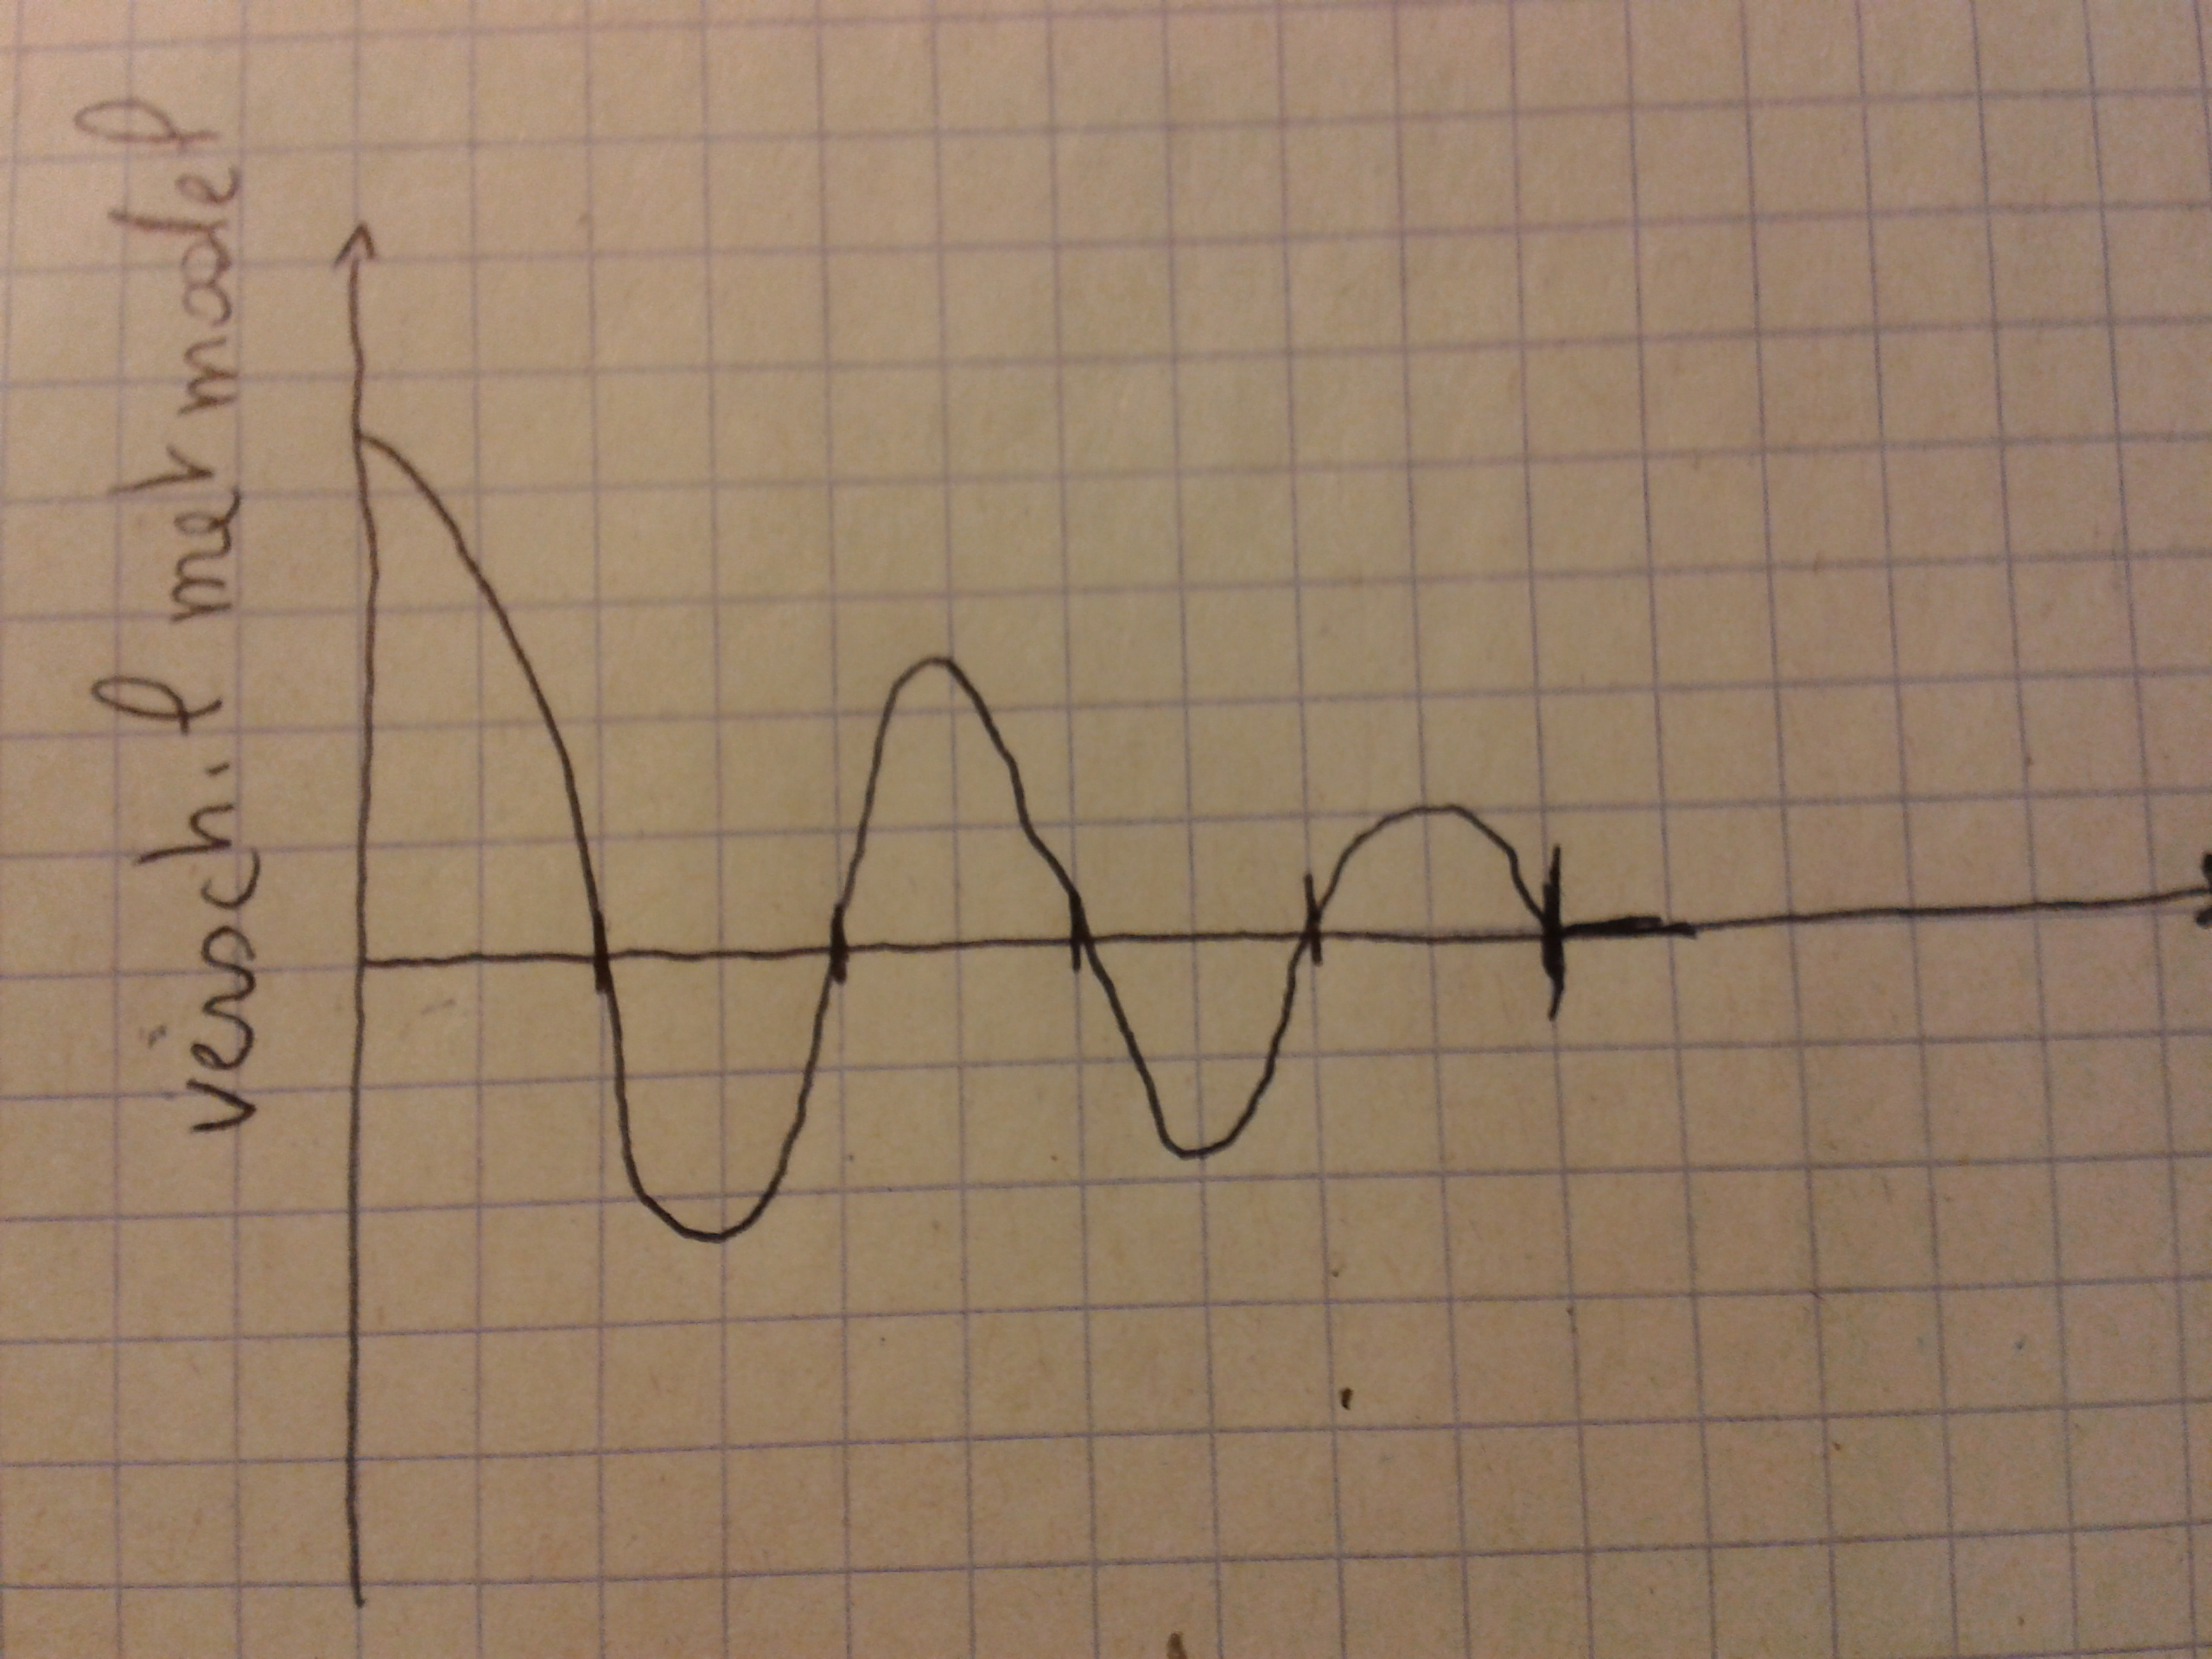
\includegraphics[width=0.6\textwidth]{images/convergentie.png}
    \caption{Grafische voorstelling van de convergentie na een reeks deployment runs.}
    \end{center}
\end{figure}

%CMS laat vaak toe om logisch samenhorende basisobjecten te verzamelen en   
Databases en webserver zijn abstracties die bestaan uit een verzameling basisobjecten zoals bestanden, packages en services.
Tussen deze objecten bestaan er natuurlijk ook afhankelijkheden, bijvoorbeel tussen een bestand en de map waarin het staat:
als de CMS eerst probeert het bestand te cree\"eren en dan pas de map zal de deployment run slechts gedeeltelijk slagen want een bestand kan niet bestaan zonder zijn parent folder.
\begin{figure}
    \label{fig:file_dir_dep}
    \begin{center}
    \includegraphics[width=0.6\textwidth]{images/file_dir_dep.png}
    \caption{Grafische voorstelling van de afhankelijkheid tussen een bestand en zijn parent folder}
    \end{center}
\end{figure}
\todo{Hier al eventual consistency vermelden/verwijzen?}

We kunnen dus concluderen dat het vermelden van dependencies in het model het uitrolprocess significant kan verbeteren: als alle afhankelijkheden vermeld zijn is er maar 1 deployment run nodig.
\todo{snelheid nog niet vermeld. Meerdere deployments onnodig maken.}
\todo{Belang: correct gebeuren is van groot belang}

%%%%%%%%%%%%%%%%%%%%%%%%%%%%%%%%%%%%%%%%%%%%%%%%%%%%%
%          Dependencies met huidige tools           %
%%%%%%%%%%%%%%%%%%%%%%%%%%%%%%%%%%%%%%%%%%%%%%%%%%%%%
De huidige CMS laten toe om op het niveau van bestanden, packages en services afhankelijkheden te specifi\"eren.
Bij het uitrollen van een model wordt dan een volgorde opgelegd waarmee de verschillende objecten verwerkt worden.

De tools die momenteel beschikbaar zijn compileren tijdens de deployment voor elke machine hun deel van het model.
Elke machine krijgt dus informatie over wat hijzelf doet maar kan geen rekening houden met wat er op andere machines gebeurt.
Afhankelijkheden binnen \'e\'en machine verwerken is dus geen probleem maar afhankelijkheden tussen verschillende machines zijn niet mogelijk. \todo{Vermelden van workarounds}
De tools die momenteel beschikbaar zijn kunnen dus het hierboven vermelde probleem van een webserver en een database niet oplossen.
%%%%%%%%%%%%%%%%%%%%%%%%%%%%%%%%%%%%%%%%%%%%%%%%%%%%%
%          Dependencies met IMP                     %
%%%%%%%%%%%%%%%%%%%%%%%%%%%%%%%%%%%%%%%%%%%%%%%%%%%%%
IMP (Infrastructure Management Platform) is een nieuwe tool die momenteel nog in ontwikkeling is.
Een andere aanpak tijdens het deployen van een model laat toe afhankelijkheden tussen hoog-niveau objecten te specifi\"eren:
in tegenstelling tot de vorige tools krijgt elke machine het volledige model ter beschikking en niet alleen zijn eigen deel.
Dit laat de machines toe om rekening te houden met afhankelijkheden tussen eigen objecten en die op een andere machine.

%%%%%%%%%%%%%%%%%%%%%%%%%%%%%%%%%%%%%%%%%%%%%%%%%%%%%
%          Probleem/doelstelling                    %
%%%%%%%%%%%%%%%%%%%%%%%%%%%%%%%%%%%%%%%%%%%%%%%%%%%%%
De doelstelling van deze thesis is een effici\"ente manier vinden om een configuratiemodel uit te rollen.
Effici\"ent slaat hier vooral op het vermijden van extra deployment runs door rekening te houden met al dan niet impliciete afhankelijkheden.

%%%%%%%%%%%%%%%%%%%%%%%%%%%%%%%%%%%%%%%%%%%%%%%%%%%%%
%          Kort: hoe oplossing + resultaten         %
%%%%%%%%%%%%%%%%%%%%%%%%%%%%%%%%%%%%%%%%%%%%%%%%%%%%%

\zexternaldocument{evaluatie}
\zexternaldocument{inleiding}

\chapter{Naar het automatisch toevoegen van vereisten en afhankelijkheden}
\label{sec:afhankelijkheden}
Configuratiebeheergereedschappen die gebruik maken van vereisten en afhankelijkheden reduceren daarmee het aantal deployment runs dat nodig is om een stabiele toestand te bereiken.
Dit hoofdstuk introduceert enkele heuristieken die ,naast degene die de gebruiker specificeert, extra vereisten en afhankelijkheden probeert toe te voegen.

Secties \ref{sec:bestanden_en_mappen}, \ref{sec:stacks} en \ref{sec:namen} introduceren heuristieken die extra vereisten toevoegen aan het model en zo het aantal fouten reduceren.

De heuristieken uit secties \ref{sec:relaties} en \ref{sec:vereisten_uit_afhankelijkheden} werken samen om afhankelijkheden om te zetten in vereisten om zo een effici\"entere volgorde opleggen aan het uitrolproces.  

\section{Vereisten tussen bestanden en mappen}
\label{sec:bestanden_en_mappen}
Deze heuristiek zorgt dat elk bestand zijn bovenliggende map vereist.
Een bestand moet namelijk deel uitmaken van een map.
Figuur \ref{fig:file_dir_dep} geeft hiervan een visuele voorstelling.

Het algoritme dat hiervoor gebruikt wordt ziet eruit als volgt (pseudocode):
\begin{minipage}{\textwidth}
\begin{lstlisting}[language=Python]
for file in host.resources:
    for dir in host.resources:
        if get_directory(file.path) == dir.path:
            file.requires.add(dir)
\end{lstlisting}
\end{minipage}

Als de map niet vermeld wordt in het model wordt deze ook niet toegevoegd omdat dit ongewenste gevolgen kan hebben. \todo{Welke?}

\section{Vereisten tussen services, packages en configuratiebestanden}
\label{sec:stacks}
Net zoals bij bestanden en mappen zijn er voorwaarden voor het correct uitrollen van packages, services en hun eventuele configuratiebestanden:
een service kan niet starten als zijn package niet ge\"installeerd is en zal niet correct werken zonder een aangepast configuratiebestand.
De verzameling van een service, het pakket dat die service installeert en de configuratiebestanden wordt vanaf nu een stack genoemd.
Een schematische voorstelling van de onderlinge vereisten bnnen een stack is te vinden op figuur \ref{fig:stack}.

\begin{figure}[h]
    \begin{center}
    \includegraphics[width=0.6\textwidth]{images/stack.pdf}
    \caption{Grafische voorstelling van de onderlinge vereisten van packages, services en configuratiebestanden binnen een stack}
    \label{fig:stack}
    \end{center}
\end{figure}

Een eerste aanpak om de correcte afhankelijkheden te introduceren is alle pakketten en bestanden een vereiste maken van alle services en alle pakketten een vereiste van alle bestanden.
De configuratiebestanden mogen pas geplaatst worden nadat de packages ge\"installeerd zijn omdat anders het aangepast configuratiebestand overschreven wordt.
Dit introduceert uiteraard veel afhankelijkheden die niet overeenstemmen met de werkelijkheid maar ze maken daardoor het resultaat van het uitrolproces niet fout.
Als het model maar \'e\'en stack bevat voegt de heuristiek geen enkele overbodige vereiste toe, bij twee stacks zes overbodige vereisten, bij drie stacks 27,\ldots
Een algoritme in pseudocode ziet er uit als volgt:

\begin{minipage}{\textwidth}
\begin{lstlisting}[language=Python]
for service in host.resources:
    for file in host.resources:
        service.requires.add(file)
    for package in host.resources:
        service.requires.add(package)
for file in host.resources:
    for package in host.resources:
        file.requires.add(package)
\end{lstlisting}
\end{minipage}

Deze heuristiek resulteert in een soort batchuitvoering waarbij de CMS  eerst alle pakketten installeert, dan alle (configuratie)bestanden en uiteindelijk alle services.

De volgende aanpak gebruikt meer info uit het model en resulteert in minder overbodige afhankelijkheden.
In de modelcode worden bestanden, packages en services die bij elkaar horen meestal binnen eenzelfde implementatie gespecifi\"eerd.
Een voorbeeld is de implementatie van een MySQL server:

\begin{minipage}{\textwidth}
\begin{lstlisting}
implementation mysql:
    pkg = std::Package(host= host, name= "mysql-server", state= "installed")
    svc = std::Service(host= host, name= "mysqld", state= "running", onboot= true)

    config= std::ConfigFile(host= host, path= "/etc/my.cnf", content= template("mysql/my.cnf.tmpl"), requires= pkg, reload= true)
    conf_dir= std::Directory(host= host, path= "/etc/mysql.conf.d", owner= "root", group= "root", mode= 755)

    dblist= std::ConfigFile(host= host, path= "/etc/sysconfig/mysql", reload= true, content= template("mysql/databases.tmpl"))
end
\end{lstlisting}
\end{minipage}

Bij het verwerken van het model tijdens het uitrolproces zijn de resources van deze stack binnen \'e\'enzelfde scope gedefini\"eerd.
De heuristiek zoekt verzamelingen van packages en services die binnen \'e\'enzelfde scope gedefini\"eerd zijn en stelt de correcte afhankelijkheden op tussen enkel die groep resources.
De aanwezigheid van files is optioneel: sommige services hebben geen aangepast configuratiebestand nodig.

\begin{minipage}{\textwidth}
\begin{lstlisting}
srv_stacks = []
for resource in resources:
    same_scope = [res in resources where res.scope == resources.scope]
    if same_scope.contains(services) and same_scope.contains(packages):
        srv_stacks.add(same_scope)

for stack in srv_stacks:
    for service in stack:
        for file in stack:
            service.requires.add(file)
        for package in stack:
            service.requires.add(package)
    for file in stack:
        for package in stack:
            file.requires.add(package)
\end{lstlisting}
\end{minipage}

Deze heuristiek voegt geen overbodige vereisten toe, op voorwaarde dat degene die het model opstelt de verschillende stacks opsplitst in verschillende implementaties.
Resultaten van het gebruik van deze heuristiek staan in sectie \ref{sec:stacks_eval}.

\section{Vereisten tussen resources met gelijkaardige naam}
\label{sec:namen}
De laatste heuristiek heeft een gelijkaardige doel als de vorige: vereisten opstellen tussen de onderdelen van een stack.
In plaats van te werken binnen een scope zoekt deze heuristiek naar resources met een gelijkaardige naam.

In het geval van de vereisten tussen bestanden en pakketten negeert de heuristiek de cijfers op het einde van de naam van een pakket en als er een splitsingsteken staat in de naam houdt het enkel rekening met het eerste deel.
Zo stelt de heuristiek ook afhankelijkheden op tussen bijvoorbeeld het pakket ``cassandra12'' en het configuratiebestand ``/etc/cassandra.conf'' of het pakket ``openssh-server'' en ``/etc/openssh.conf''. 

Namen gebruiken levert meer vereisten op dan het gebruik van scopes.\todo{Uitleggen waarom}

\begin{minipage}{\textwidth}
\begin{lstlisting}
for service in host.resources:
    similar_resources = []
    for file in host.items:
        if file.name.contains(service.name):
            service.requires.add(file)
    for package in host.items:
        if package.name.contains(service.name):
            service.requires.add(package)

for package in host.resources:
    name = remove_digits(package.name)
    name = name.split("-")[0]
    for file in host.items:
        if file.name.contains(service.name):
            package.requires.add(file)
\end{lstlisting}
\end{minipage}

\section{Afhankelijkheden door relaties}
\label{sec:relaties}
IMP laat toe relaties tussen concepten te modelleren.
Een voorbeeldrelatie is de volgende:
\begin{lstlisting}
BaseClient clients [0:] -- [0:] BaseServer servers
\end{lstlisting}
Deze betekent dat een BaseClient nul of meerdere BaseServers nodig heeft, en omgekeerd.
Een ander voorbeeld is 
\begin{lstlisting}
Host host [1] -- [0:] File files
\end{lstlisting}
Dit betekent dat op een Host nul of meerdere files kunnen staan, maar dat elke File \'e\'en Host moet hebben.
Deze heuristiek leidt hieruit af dat een File niet kan bestaan zonder een host en het dus nodig is dat eerst de Host uitgerold wordt voordat geprobeerd wordt de File te cree\"eren.

Algemeen kan men dus besluiten dat elke relatie waar de ene kant een multipliciteit van [0] of [0:] heeft en de andere kant multipliciteit [n] of [n:] de eerste entiteit afhankelijk is van de tweede.
De code voor deze heuristiek ziet er uit als volgt:

\begin{minipage}{\textwidth}
\begin{lstlisting}
for lib in model.get_scopes():
    for concept in lib.variables():
        if concept.hasattr(relation)
            if concept.relation.low == 0 and concept.relation.end == 1:
                concept.relation.depends = True
\end{lstlisting}
\end{minipage}

Als enkel deze heuristiek gebruikt wordt zal IMP niets veranderen aan het uitrolproces: IMP houdt momenteel nog geen rekening met afhankelijkheden.
De extra informatie kan wel gebruikt worden door andere heuristieken.
Een voorbeeld hiervan is deze hieronder (sectie \ref{sec:vereisten_uit_afhankelijkheden}) die toelaat afhankelijkheden zoals deze tussen een webserver en databaseserver te gebruiken voor een optimaler uitrolproces.

\section{Vereisten vanuit afhankelijkheden}
\label{sec:vereisten_uit_afhankelijkheden}
IMP laat niet alleen toe om afhankelijkheden tussen enkelvoudige concepten zoals bestanden, services,\ldots te specifi\"eren maar ook tussen samengestelde concepten zoals webservers, databaseservers,\ldots
Deze betekenen dat de ene kant niet zijn volledige functionaliteit kan aanbieden zonder de aanwezigheid van de andere kant.
Aangezien een server zijn functionaliteit aanbiedt aan de hand van een service en niet zijn configuratiebestanden en pakketten stelt deze heuristiek enkel afhankelijkheden op tussen de services.

IMP laat toe om verschillende libraries te gebruiken (en zelf te defini\"eren) met daarin voorgedefinieerde concepten. 
Het algoritme begint met het doorzoeken van deze libraries naar concepten die services bevatten.
Dan kijkt het of dat concept afhankelijk is van een ander concept.
Als dit het geval is wordt gekeken of dat ander concept ook services bevat.
Zo ja stelt de heuristiek vereisten op tussen de services. 

In pseudocode ziet dit er uit als volgt:

\begin{minipage}{\textwidth}
\begin{lstlisting}
for lib in model:
    for concept in lib.variables():
        concept_services = get_services(concept)
        if concept_services is not None:
            for relation in concept.get_attributes():
                if relation.depends: #afhankelijke relatie
                    for instance in concept.values: #Voor elke instantie v/h concept
                        req_concepts = relation.end
                        req_resources = []
                        for req_concept in req_concepts:
                                for srv in get_services(req_concept):
                                    req_resources.add(srv)
                        if req_resources is not None: 
                            for service in concept_services:
                                for req_res in req_resources:
                                    service.requires.add(req_res)
\end{lstlisting}
\end{minipage}

Het is belangrijk dat deze heuristiek wordt opgeroepen na deze van sectie \ref{sec:relaties}, daar worden namelijk extra afhankelijke relaties opgesteld die hier kunnen gebruikt worden.

\section{Besluit van dit hoofdstuk}



\zexternaldocument{inleiding}
\zexternaldocument{analyse}
\zexternaldocument{imp}

\chapter{Evaluatie}
\label{sec:evaluatie}
Om de impact van de verschillende heuristieken te meten volgt nu een overzicht van de testresultaten.
Voor het merendeel van de testen is een simulator gebruikt.
Sectie \ref{sec:simulator} legt uit waarom een simulator gebruikt wordt in plaats van IMP zelf, en hoe deze werkt.

De daarop volgende secties bespreken de resultaten van elke heuristiek. 
De algemene verwachting is dat het gebruik van heuristieken het aantal deployment runs reduceert en zo ook de totale uitroltijd.
Deze optimalisatie kost wel extra verwerkingstijd (de uitvoering van de verschillende heuristieken) maar deze is normaal gezien te verwaarlozen ten opzichte van het volledige uitrolproces.\todo{meten} 

\section{Simulator}
\label{sec:simulator}
Als deel van deze thesis werd een simulator voor IMP ontwikkeld.
Deze heeft een belangrijk aandeel in het evalueren van de ontwikkelde heuristieken.
Ze laat namelijk toe op een snelle en eenvoudige manier een uitgebreid model uit te rollen en geeft volledige controle over welke informatie tijdens dat proces beschikbaar wordt gesteld aan de gebruiker.
De snelheid en eenvoud van de simulator in vergelijking met op fysieke hosts uitrollen is te danken aan twee redenen:

ten eerste is de uitroltijd evenredig met het aantal resources in het model.
Elke resource moet verwerkt worden, en vooral pakketten duren lang om uit te rollen. 
Deze moeten niet alleen gedownload worden maar ook ge\"installeerd, beide taken kunnen aardig wat tijd innemen.
Bij de simulator komt het uitrollen van een pakket overeen met het wegschrijven van een reeks waarden in een database, wat significant sneller is.
Hierbij moet wel een kanttekening gemaakt worden: bij fysiek uitrollen wordt het uitrollen van het model verdeeld over de verschillende hosts, elk zijn eigen deel van het model.
De simulator moet alle resources van alle hosts alleen verwerken. 
Zelfs dan nog is de snelheidswinst bij de simulator significant.

Ten tweede laat een simulator toe modellen met honderden machines uit te rollen op \'e\'en enkele pc.
Naarmate de modellen groter worden wordt het steeds moeilijker het model op fysieke hosts te testen.
En het zijn juist de grotere modellen, met meer hosts, die interessant zijn voor de evaluatie van de heuristieken.

De simulator bootst een systeem na dat Fedora 18 draait en gebruik maakt van de yum pakket manager.

\subsection{Uitwerking}
\label{simulator:uitwerking}
De simulator is een Pythonscript dat als invoer een JSON-bestand met daarin het gecompileerde model.
IMP zelf stelt dit bestand op als de optie ``-j [naam JSON]'' wordt meegegeven.
Tijdens het uitvoeren van dit script wordt een sqlite-database opgesteld.
De tabellen van deze database zijn te zien in de tabellen \ref{table:deploymentdatabase}.

\begin{table}[h]
\centering
\begin{tabular}[t]{ |l|l| }
  \hline
  \multicolumn{2}{|c|}{Agent} \\
  \hline
  name & Text \\
  \hline
\end{tabular}
\quad
\begin{tabular}[t]{ |l|l| }
  \hline
  \multicolumn{2}{|c|}{Attribute} \\
  \hline
  name & Text \\
  value & Text \\
  ResourceId & Text \\
  \hline
\end{tabular}
\quad
\begin{tabular}[t]{ |l|l| }
  \hline
  \multicolumn{2}{|c|}{Resource} \\
  \hline
  Id & Text \\
  \hline
\end{tabular}
\caption{De verschillende tabellen die aanwezig zijn in de deploymentdatabase.}
\label{table:deploymentdatabase}
\end{table}

In de Attribute tabel staan de attributen opgeslagen als volgt:
\begin{verbatim}
name     value       ResourceId                                                                                          
-------- ---------- ---------------------------------------------------
group    root        std::File[server,path=/tmp/test],v=1389435342             
owner    root        std::File[server,path=/tmp/test],v=1389435342             
path     /tmp/test   std::Directory[server,path=/tmp/test],v=1389435342                        
\end{verbatim}

Om de simulatie zo waarheidsgetrouw mogelijk te maken houdt de simulator rekening met volgende aspecten van het fysieke uitrolproces:

\begin{itemize}
  \item Bestanden en mappen kunnen niet aangemaakt worden voordat de bovenliggende map bestaat.
  \item Services kunnen niet gestart worden voordat het bijhorende pakket en bestanden aanwezig zijn.
  \item Resources worden pas aangemaakt als hun afhankelijkheden voldaan zijn.
\end{itemize}

Nakijken of alle bijhorende pakketten en bestanden van een service aanwezig zijn wordt gebruikt gemaakt van de repositorydata van de yum pakketmanager.
De repositorydata bevat twee handige databases: de primary en de filelists.
De relevante attributen de gebruikte tabellen zijn te vinden in tabel \ref{table:repodata}.

\begin{table}[h]
\centering
\begin{tabular}[t]{ |l|l| }
  \hline
  \multicolumn{2}{|c|}{packages} \\
  \hline
  pkgKey & Integer \\
  name & Text \\
  \hline
\end{tabular}
\quad
\begin{tabular}[t]{ |l|l| }
  \hline
  \multicolumn{2}{|c|}{filelist} \\
  \hline
  pkgKey & Integer \\
  name & Text \\
  dirname & Text \\
  filenames & Text \\
  \hline
\end{tabular}
\caption{De relevante attributen van de repositorydatabases die gebruikt worden door de simulator}
\label{table:repodata}
\end{table}

De uiteindelijke database die gebruikt wordt door te simulator bestaat uit de samenvoeging van de attributen uit de twee databases.
Aangezien sommige pakketten een eigen yum repository hebben is voor die gevallen manueel de repositorydata toegevoegd.
Een voorbeeld van de data die zo bekomen wordt:

\begin{verbatim}
name          dirname                    filenames                     
------------  -------------------------  ------------------------------
oniguruma     /usr/lib                   libonig.so.2.0.0/libonig.so.2 
oniguruma     /usr/share/doc             oniguruma-5.9.2               
openCOLLADA   /usr/share/doc             openCOLLADA-0                 
\end{verbatim}

Bij het installeren van een pakket in de simulator wordt een lijst van alle bestanden en mappen die bij dat pakket horen opgesteld.
Elk element van deze lijst wordt als entry toegevoegd aan de Attribute tabel, met als value het pad naar dat bestand.
Als de simulator probeert een bepaalde service uit te rollen zoekt hij alle entries met de servicenaam en stelt een lijst met alle nodige bestanden en mappen op.
Daarna wordt in de Attribute tabel gecheckt of deze allemaal aanwezig zijn.

Naast de repositorydata wordt ook nog een lijst gebruikt met daarin de bestanden en mappen die standaard aanwezig zijn op een nieuwe Fedora 18 installatie.
Zonder deze lijst zou elke poging tot het uitrollen van een bestand of map falen, omdat voor geen enkel bestand de bovenliggende map bestaat.

In pseudecode ziet het uitrollen van elke type resource er uit als volgt:

\begin{lstlisting}[showstringspaces=false]
def deploy_file(file):
  #Check if parent folder exists already
  if parent(file) in std_filesystem or parent(file) in deployment_database:
    deployment_database.write(file)
  else:
    error('Parent folder doesn't exist!')

def deploy_service(srv):
  #Check if required files have been deployed
  requirements = repodata_database.execute('select * from pkgdata where name like srv.name')
  if all([req in deployment_database for req in requirements]):
    deployment_database.write(srv)
  else:
    error('Not all required resources were deployed!')

def deploy_package(pkg):
  pkg_files = repodata_database.execute('select * from pkgdata where name like pkg.name') 
  foreach file in pkg_files:
    deployment_database.write(file)
\end{lstlisting}

Bij het uitrollen van een pakket worden geen controles gedaan. 
De simulator gaat er van uit dat het correct uitrollen van een pakket de verantwoordelijkheid is van de pakketmanager, niet de CMS.

Om zo goed mogelijk een fysiek uitrolproces te simuleren gebruikt de simulator een gelijkaardig algoritme voor het uitrollen van het model.
Daarbij worden eerst alle resources weggeschreven die geen vereisten hebben.
Daarna wordt gekeken of de resources die net zijn uitgerold een vereiste waren van de overblijvende resources.
Als dit het geval is worden de geschreven resources verwijderd uit de lijst met vereisten.
Zo komen (hopelijk) nieuwe resources vrij die geen vereisten meer hebben en die kunnen in de volgende herhaling uitgerold worden.
Dit proces herhaalt zich tot er geen resources meer moeten uitgerold worden.

\todo{Verschil in uitroltijd simulator/IMP?}
\todo{Besluit sectie}

\section{Afhankelijkheden tussen bestanden en mappen}
\label{sec:bestanden_en_mappen_eval}
Aangezien een bestand niet kan gecre\"eerd worden zonder zijn bovenliggende map voegt deze heuristiek automatisch de afhankelijkheid tussen beide toe aan het model.

Aangezien mappen altijd kunnen gecre\"eerd worden zijn er maximaal twee deployment runs nodig als er geen heuristiek gebruikt wordt.\footnote{Twee runs als maar \'e\'en bovenliggende map moet aangemaakt worden. Per bijkomend niveau is mogelijks een extra run nodig.}
Bij gebruik van de heuristiek moet er exact \'e\'en uitgerold worden.
De verwachting is dat het uitrollen met gebruik van de heuristiek dan ook ongeveer half zo lang duurt.

Figuur \ref{fig:file_dir_times} toont de resultaten van deze test.
Elk datapunt is het gemiddelde van 30 runs, uitgevoerd op een virtuele machine met twee cores van 2Ghz en 2GB RAM ter beschikking.
Het model bestaat iedere keer uit een vast aantal bestanden en mappen, \'e\'en bestand per map.
\begin{figure}[h]
    \begin{center}
    \includegraphics[width=0.8\textwidth]{images/file_dir_times.pdf}
    \caption{Testresultaten bij het uitrollen van een stijgend aantal bestanden en mappen, met en zonder gebruik van de heuristiek}
    \label{fig:file_dir_times}
    \end{center}
\end{figure}

De verwachtingen zijn volledig ingelost: zonder heuristiek zijn er twee deployment runs nodig, met heuristiek slechts \'e\'en.
Dit weerspiegelt zich in de gehalveerde uitroltijd.

\section{Afhankelijkheden tussen services, pakketten en configuratiebestanden}
\label{sec:stacks_eval}
De specificatie van een service in het configuratiemodel gaat vaak gepaard met de pakket en de configuratiebestanden die die service nodig heeft.
Deze combinatie van resources wordt een stack genoemd.
Aangezien de service niet correct werkt zonder de aanwezigheid van het pakket en de configuratiebestanden voegt deze heuristiek de gepaste vereisten toe aan het model.


Voor deze test moest IMP 30 keer de NTP service uitrollen op een testmachine.
NTP bestaat uit \'e\'en pakket, \'e\'en configuratiebestand en \'e\'en service. 
In het slechtste geval zijn er normaal gezien dus drie deployment runs nodig om de service correct werkende te krijgen.
Als de correcte afhankelijkheden worden opgesteld is er slechts \'e\'en run nodig.
De testresultaten zijn te vinden in tabel \ref{table:service_package_dep}.

\begin{table}
  \begin{center}
  \begin{tabular}{ r | c | c }
            & tijd(s)   & gemiddeld aantal runs nodig \\ \hline
    zonder  & 3.21      & 2.0 \\ \hline
    met     & 2.21      & 1 \\
  \end{tabular}
  \caption{Meetresultaten}
  \label{table:service_package_dep}
  \end{center}
\end{table}
%specifieke resultaten:
%zonder
%Avg time: 3.212880388398965
%Deployments avg: 2.0
%met: Avg time: 2.2067235755423704
%deps toegevoegd: 3

De resultaten van de test zijn zoals verwacht: dankzij de heuristiek is maar \'e\'en deployment run nodig.

\section{Relaties en afhankelijkheden tussen hoog-niveau concepten}
De heuristieken uit sectie \ref{sec:relaties} en \ref{sec:vereisten_uit_afhankelijkheden} werken best samen.
De eerste vormt relaties met een bepaalde multipliciteit om naar afhankelijke relaties.
De tweede zet afhankelijke relaties tussen entiteiten die services bevatten om naar vereisten tussen die services.
Zo wordt vermeden dat een extra deployment run nodig is de services correct op te starten.

Deze heuristieken werden niet apart getest, enkel in de use cases.
In individuele testen zouden de resultaten gelijkaardig zijn aan die van de bestanden en mappen heuristiek.

\section{Use cases}

\subsection{Document processing}
Deze eerste use case studie betreft een uitgebreide en complexe infrastructuur gebruikt voor de geautomatiseerde verwerking van documenten.
De infrastructuur ondersteunt \todo{cite} de creatie, het opstellen van de layout, de processing en het opslaan van bedrijfsdocumenten (bvb facturen, orders, aandelen,\ldots).
Ze wordt meestal uitgerold als een cloudservice.
Figuur \ref{fig:doc_processing} toont de verschillende onderdelen van deze opstelling:
de gebruiker kan via verschillende inputkanalen data doorspelen aan de productieservice.
Die verwerkt de gegevens in verschillende stappen.
De worker nodes zijn verantwoordelijk voor de verwerking van die acties.
De resultaten worden geplaatst in een database en kunnen via verschillende outputkanalen opgevraagd worden.

\begin{figure}[h]
    \begin{center}
    \includegraphics[width=0.8\textwidth]{images/doc_processing.pdf}
    \caption{Overzicht van de document processing infrastructuur}
    \label{fig:doc_processing}
    \end{center}
\end{figure}

Het volledige model in IMP van deze use case bestaat uit 35 bibliotheken \todo{bibliotheken vermelden, mogelijks een hoofdstuk introductie tot IMP?} waaronder Apache, HBase, Cassandra, \ldots
In totaal zijn er reeds 82 relaties gespecifi\"eerd, maar het model is nog niet volledig.

\todo{Dit is eigenlijk geen uitleg van de toepassing van de heuristieken op de use case, meer een uitleg/test van de heuristieken}
In afbeelding \ref{fig:reqs_doc} is te zien hoeveel vereisten elke heuristiek toevoegen.
De heuristiek die de bovenliggende map toevoegt aan de vereisten van een map of bestand wordt altijd uitgevoerd.
Deze heuristiek beschouwen we namelijk als fundamenteel: de vereisten die ze toevoegd zijn sowieso juist, terwijl sommige vereisten die door andere heuristieken worden toegevoegd mogelijks overbodig zijn. 

De verwachting is dat sommige heuristieken zullen overlappen, bijvoorbeeld ``stack'' en ``name''. 
Resources binnen dezelfde stack hebben namelijk vaak een gelijkaardige naam. 

\begin{figure}[h]
    \begin{center}
    \includegraphics[width=0.8\textwidth]{images/reqs_doc.pdf}
    \caption{Aantal toegevoegde vereisten voor elke combinatie van heuristieken in de document processing use case}
    \label{fig:reqs_doc}
    \end{center}
\end{figure}

Als een bepaalde heuristiek eerst toegepast wordt kan hij al zijn vereisten toevoegen.
Daaropvolgende heuristieken zullen enkel het deel van hun vereisten toevoegen die nog niet deel uitmaken van het model.
Ongeacht de volgorde zal een combinatie heuristieken altijd dezelfde set vereisten toevoegen.

In afbeelding \ref{fig:time_runs_doc} is te zien welke impact de toegevoegde vereisten hebben op het uitrolproces.

\begin{figure}[h]
    \begin{center}
    \includegraphics[width=0.8\textwidth]{images/time_runs_doc.pdf}
    \caption{Gemiddelde aantal uitgerolde resources per deployment run voor elke combinate van heuristieken in de document processing use case}
    \label{fig:time_runs_doc}
    \end{center}
\end{figure}

De resultaten bevestigen onze aanname dat het toevoegen van vereisten kan leiden tot een daling in het aantal deployment runs.
Elke combinatie van de drie heuristieken leidt zelfs tot een ``one-shot'' uitrolproces waarin in \'e\'en keer het volledige model correct uitgerold wordt.

Het volledige model bevat 82 relaties. 
\subsection{MongoDB}
MongoDB is een van de meer bekende NoSQL databases.
Een volledige configuratie bestaat uit verschillende services die elkaar ondersteunen.
Figuur \ref{fig:mongodb_architecture} geeft een schematische voorstelling van een dergelijke set-up. \todo{cite}

\begin{figure}[h]
    \begin{center}
    \includegraphics[width=0.8\textwidth]{images/mongodb_architecture.pdf}
    \caption{Architectuur van de MongoDB database}
    \label{fig:mongodb_architecture}
    \end{center}
\end{figure}

In het model dat Thomas Uyttendaele opgesteld heeft \todo{cite} krijgen de onderdelen de volgende namen:

\begin{table}[h!]
  \begin{center}
  \begin{tabular}{c | c}
  Query Router  & AccessServer \\ \hline
  Primary       & ReplicaSetController \\ \hline
  Secondary     & Node \\ 
  \end{tabular}
  \end{center}
\end{table}

De onderdelen zullen pas correct kunnen samenwerken als ze in de juiste volgorde worden opgestart.
Figuur \ref{fig:mongo_imp} toont de implementatie van MongoDB in IMP, samen met de volgorde waarin de services gestart moeten worden.

\begin{figure}[h]
    \begin{center}
    \includegraphics[width=0.8\textwidth]{images/mongo_imp.pdf}
    \caption{Implementatie van MongoDB in IMP, met de correcte opstartvolgorde aangeduid}
    \label{fig:mongo_imp}
    \end{center}
\end{figure}

Het is dus weerom \todo{Vroeger vermelden dat het van groot belang is dat het model compleet is} van groot belang dat alle afhankelijkheden in het model
vermeld worden.

Voor de volgende resultaten werd een instantie van MongoDB uitgerold met vijf nodes, verdeeld in twee replicasets van twee en drie nodes elk.
Drie nodes nemen ook de rol van Query Router op zich.
Figuur \ref{fig:reqs_mongo} toont de vereisten die elke combinatie van heuristieken toevoegt.

\begin{figure}[h]
    \begin{center}
    \includegraphics[width=0.8\textwidth]{images/reqs_mongo.pdf}
    \caption{Aantal toegevoegde vereisten voor elke combinatie van heuristieken bij MongoDB}
    \label{fig:reqs_mongo}
    \end{center}
\end{figure}

Figuur \ref{fig:time_runs_mongo} toont hoeveel deployment runs nodig zijn om een volledig werkende MongoDB database te bekomen, en hoeveel resources er
per run gedeployed worden.

\begin{figure}[h]
    \begin{center}
    \includegraphics[width=0.8\textwidth]{images/time_runs_mongo.pdf}
    \caption{Gemiddelde aantal uitgerolde resources per deployment run voor elke combinate van heuristieken bij MongoDB}
    \label{fig:time_runs_mongo}
    \end{center}
\end{figure}

De library voor MongoDB bestaat uit 185 regels code\footnote{Blanco lijnen en commentaar niet meegerekend}, waarvan er 24 relaties beschrijven.
Alle libraries samen bevatten 50 relaties. 

\chapter{Besluit}
\label{sec:besluit}

\section{Gerelateerd werk}
\todo{verwijzen naar overzichtspaper}
Cloud Resource Orchestration: A Data-Centric Approach: andere aanpak om te vermijden dat inconsistente configuraties bereikt worden.
Datacentrische aanpak (declaratief) itt tot andere tools die heel imperatief werken (bvb ansible)

\todo{IBM}

\section{Verder werk}
%Meer use cases%
Een eerste onderzoeksrichting betreft de heuristieken.
Niet alleen worden deze beter nog in andere use cases gebruikt om hun validiteit verder te bevestigen, nieuwe use cases kunnen ook leiden tot nieuwe heuristieken.

De heuristieken kunnen mogelijks ook gebruikt worden als onderdeel van een intelligente autocompletetool. 
Een dergelijke tool stelt de gebruiker voor om vereisten tussen resources binnen een stack toe te voegen, of suggereert om bepaalde relaties als afhankelijk te specificeren.

%kijken welke subset van deps nu echt nodig is.%
Verder onderzoek kan ook pogen de minimale set vereisten te defini\"eren die nodig is om een model correct uit te rollen.
De heuristieken die voortkomen uit dit onderzoek voegen liever een extra vereiste toe dan geen.
Deze aanpak is goed zolang er geen incorrecte of overbodige vereisten worden toegevoegd, maar elke vereiste moet verwerkt worden door IMP.
Dit zorgt voor een kleine verhoging in de uitvoertijd.
Een minimale set vereisten kan dus een positief effect hebben op de totale uitroltijd.

%Deletes%
Een derde richting die verder onderzocht kan worden is hoe IMP (of CMS in het algemeen) kan omgaan met verschillende tussen opeenvolgende versies van een configuratiemodel.
Momenteel stopt alle CMS dan met het onderhoud van die resource. 
In sommige gevallen kan dit ongewenste gevolgen hebben: een database die online blijft maar een niet meer geupdated wordt is een veiligheidsrisico.
De service stoppen als ze niet meer in het model vermeld staat zou hier een betere optie zijn.
Mogelijks leidt dit zelfs tot andere resources die overbodig worden, zoals een database die enkel gebruikt door een webserver.
Als de webserver uitgeschakeld wordt kan het wenselijk zijn om automatisch ook de databaseserver stop te zetten.
Dit soort acties zijn mogelijk in IMP omdat in het model de relaties staan die aanwezig zijn in de opstelling.


% Indien er bijlagen zijn:
\appendixpage*          % indien gewenst
\appendix
\chapter{Code van de heuristieken}
\label{app:code}
\section{Bestanden en mappen}
\begin{minipage}{\textwidth}
\begin{lstlisting}[language=Python]
def dir_before_file(model, resources):
    for _id, resource in resources.items():
        model = resource.model
        res_class = model.__class__
        if model.__module__ == "std" and (res_class.__name__ == "File" or res_class.__name__ == "Directory"):
            host = model.host
 
            for dir in host.directories:
                dir_res = Resource.get_resource(dir)
                if dir_res is not None and os.path.dirname(resource.path) == dir_res.path:
                    if dir_res.id not in resource.requires:
                        resource.requires.add(dir_res.id)
\end{lstlisting}
\end{minipage}

\section{Services, packages en configuratiebestanden}
\subsection{Methode 1}
\begin{minipage}{\textwidth}
\begin{lstlisting}[language=Python]
TODO: herschrijven
\end{lstlisting}
\end{minipage}

\subsection{Methode 2}
\begin{minipage}{\textwidth}
\begin{lstlisting}
def scope_dependencies(model, resources):
    srv_stacks = find_srv_stacks(resources)
    deps_per_stack = [] 
    for stack in srv_stacks:
        deps_per_stack.append(setup_stack_deps(stack))
 
def find_srv_stacks(resources):
    stacks = []
    for res in resources.values():
        scope_pkg = []
        scope_cfg = []
        scope_srv = []
        model_instance = res.model
        instance_scope = model_instance.__scope__
        scope_vars = instance_scope.variables()
        scope_cfg = [x.value for x in scope_vars if x.value.__class__.__name__ == "File"]
        scope_srv = [x.value for x in scope_vars if x.value.__class__.__name__ == "Service"]
        scope_pkg = [x.value for x in scope_vars if x.value.__class__.__name__ == "Package"]
 
        if scope_srv and (scope_pkg or scope_cfg):
            stacks.append({'pkg': scope_pkg, 'srv': scope_srv, 'cfg': scope_cfg})
 
    return stacks
 
def setup_stack_deps(stack):
    deps = 0
    for srv in stack['srv']:
        srv = Resource.get_resource(srv)
        for pkg in stack['pkg']:
            pkg = Resource.get_resource(pkg)
            if pkg.id not in srv.requires:
                srv.requires.add(pkg.id)
                deps = deps + 1
        for cfg in stack['cfg']:
            cfg = Resource.get_resource(cfg)
            if cfg.id not in srv.requires:
                srv.requires.add(cfg.id)
                deps = deps + 1
    for cfg in stack['cfg']:
        cfg = Resource.get_resource(cfg)
        for pkg in stack['pkg']:
            pkg = Resource.get_resource(pkg)
            if pkg.id not in cfg.requires:
                cfg.requires.add(pkg.id)
                deps = deps + 1
    return deps

\end{lstlisting}
\end{minipage}

\section{Resources met gelijkaardige namen}
\begin{minipage}{\textwidth}
\begin{lstlisting}
def name_dependencies(model, resources):
    deps = 0
    for _id, res in resources.items():
        similar_resources = []
        res_model = res.model
        if res_model.__module__ == "std" and res_model.__class__.__name__ == "Service":
            for other_id, other_res in resources.items():
                similar_reg = re.compile("std::File.*%s.*%s.*" % (res.model.host.name, res.name))
                if other_res.model.__class__.__name__ == "File" and similar_reg.match(str(other_id)):
                    similar_resources.append(other_res)
            
            for similar_res in similar_resources:
                if similar_res.id not in res.requires:
                    res.requires.add(similar_res.id)
 
        if res_model.__module__ == "std" and res_model.__class__.__name__ == "Package":
            pkg_name = ''.join(i for i in res.name if not i.isdigit())
            pkg_name = pkg_name.split("-")[0]
            for other_id, other_res in resources.items():
                similar_reg = re.compile("std::File.*%s.*%s.*" % (res.model.host.name, pkg_name))
                if other_res.model.__class__.__name__ == "File" and similar_reg.match(str(other_id)):
                    similar_resources.append(other_res)
            
            for similar_res in similar_resources:
                if res.id not in similar_res.requires and similar_res not in res.requires:
                    similar_res.requires.add(res.id)
\end{lstlisting}
\end{minipage}

\section{Afhankelijkheden door relaties}
\begin{minipage}{\textwidth}
\begin{lstlisting}
def use_rel_multiplicity(model, resources):
    added = 0
    for lib in model.get_scopes():
        for concept in lib.variables():
            if concept.get_name().startswith("Entity"):
                for attr_name in concept.value.get_all_attribute_names(): #anders niet de attr vd parents
                    attr_value = concept.value.get_attribute(attr_name)
                    if hasattr(attr_value, "end"): #Kijk of het een relatie is
                        attr_end = attr_value.end
                        if attr_end.low >= 1 and attr_end.end.low == 0 and not attr_value.depends:
                            added = added + 1
                            attr_value.depends = True 
\end{lstlisting}
\end{minipage}

\section{Vereisten door afhankelijkheden}
\begin{minipage}{\textwidth}
\begin{lstlisting}
def use_relations(model, resources):
    depends = 0
    added = 0
    for lib in model.get_scopes():
        for concept in lib.variables():
            if concept.get_name().startswith("Entity"):
                concept_services = get_services(concept)
                if concept_services is not None: #Als er geen services zijn moeten er sowieso geen deps opgesteld worden
                    for attr_name in concept.value.get_all_attribute_names(): #anders niet de attr vd parents
                        attr_value = concept.value.get_attribute(attr_name)
                        if hasattr(attr_value, "end"): #Kijk of het een relatie is
                            if attr_value.end.depends: #Kijk of het concept afhankelijk is vd andere kant
                                depends = depends + 1
                                for instance in concept.value: #Voor elke instantie v/h concept de deps opstellen
                                    req_concepts = getattr(instance, attr_name)
                                    req_resources = []
                                    if hasattr(req_concepts, 'append'): #Check if QList
                                        for req_concept in req_concepts:
                                            for srv in get_child_services(req_concept):
                                                req_resources.append(srv)
                                    else:
                                        for srv in get_services(req_concepts):
                                                req_resources.append(srv)
                                    for req_res in req_resources:
                                        for service in concept_services:
                                            if req_res not in service.requires and req_res.state != "stopped":
                                                service.requires.add(req_res)

def get_child_services(object):
    services = []
    for child_res in object._childeren:
            if child_res.__module__ == "std" and child_res.__class__.__name__ == "Service":
                services.append(Resource.get_resource(child_res))
    return services
 
def get_services(concept):
    found_services = []
    
    if hasattr(concept, "value"):
        for instance in concept.value:
            if concept.__module__ == "std" and concept.__class__.__name__ == "Service":
                found_services.append(Resource.get_resource(concept))
             
            if hasattr(instance, "_childeren"):
                found_services.extend(get_child_services(instance))
                
    if hasattr(concept, "_childeren"):
                found_services.extend(get_child_services(concept))                
 
    return set(found_services)
\end{lstlisting}
\end{minipage}


\backmatter
% Na de bijlagen plaatst men nog de bibliografie.
% Je kan de  standaard "abbrv" bibliografiestijl vervangen door een andere.
\bibliographystyle{abbrv}
\bibliography{referenties}

\end{document}

%%% Local Variables: 
%%% mode: latex
%%% TeX-master: t
%%% End: 
